\section{Introduction}\label{sec:intro}

\begin{figure}[!ht]
    \centering
    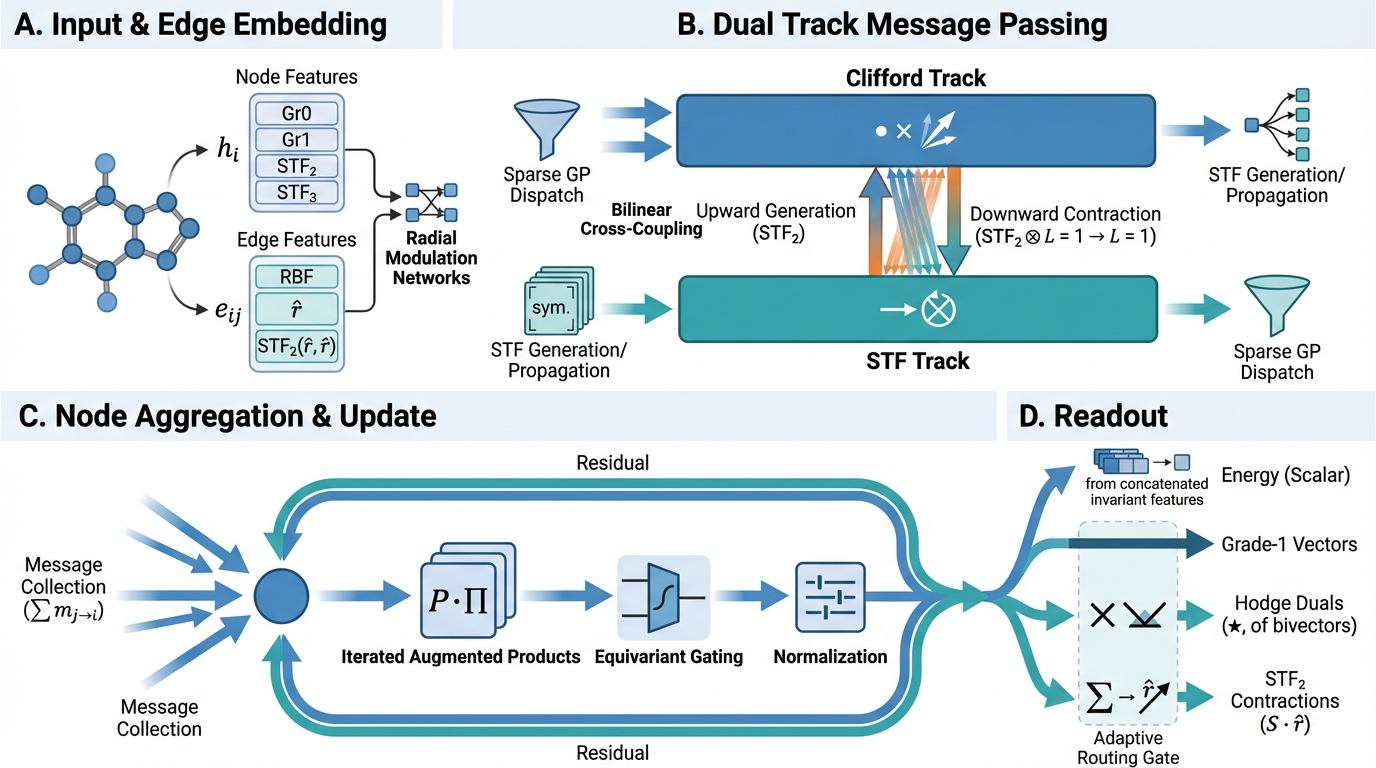
\includegraphics[width=1\linewidth]{resources/cliffordSTFMethod.png}
    \caption{\textbf{Schematic of the CliffordSTF pipeline}. (A) Atoms and edges are embedded with multivector and STF features, including explicit $L{=}2$ edge descriptors. (B) The core message-passing block uses a dual-track design where the Clifford track (geometric products) and STF track are coupled via bilinear generation and contraction operations. (C) Node updates incorporate iterated augmented products for multi-body correlations followed by equivariant gating. (D) Energy and forces are predicted from a combination of invariant and vector sources, including $L{=}2$ contractions ($S \cdot \hat{r}$) that capture angular force components inaccessible to $L \leq 1$ features.}
    \label{fig:architecture}
\end{figure}

Machine learning interatomic potentials (MLIPs) have emerged as practical surrogates for first-principles electronic structure calculations, enabling molecular dynamics at scales inaccessible to density functional theory \citep{unke2021machine}. A central design challenge is encoding the symmetries of physical law: energies must be invariant and forces equivariant under rotations and translations. The dominant approach constructs features from spherical harmonics composed through tensor products weighted by Clebsch--Gordan (CG) coefficients \citep{thomas2018tensor,batzner2022nequip,batatia2022mace}, but the computational cost of high-order couplings scales steeply with the maximum angular momentum order $L$, motivating both efficient implementations \citep{geiger2022e3nn,passaro2023escn} and CG-free reformulations based on irreducible Cartesian tensors \citep{simeon2023tensornet,zaverkin2024higher,wang2024n}.

Clifford (geometric) algebra offers an independent CG-free path. Prior architectures embed vectors into the eight-dimensional algebra $\mathrm{Cl}(3,0)$ and replace learned tensor products with the single closed-form geometric product, which handles scalars, vectors, bivectors, and pseudoscalars while preserving equivariance \citep{ruhe2023cgenn,ruhe2023gcan,brehmer2023geometric,brandstetter2022clifford}. A fundamental expressivity limitation of this substrate has nevertheless gone unacknowledged. The geometric product of two vectors in $\mathbb{R}^3$ yields a scalar and a bivector, together realising only the $L{=}0$ and $L{=}1$ components of $\mathbf{1} \otimes \mathbf{1} = \mathbf{0} \oplus \mathbf{1} \oplus \mathbf{2}$ at the per-edge bilinear used in every message-passing layer; the five-dimensional symmetric traceless $L{=}2$ component never enters the feature substrate directly. Features required for quadrupolar distributions, $d$-orbital interactions, and anisotropic stress must therefore be reconstructed indirectly through repeated products and many stacked layers, placing Clifford backbones at a systematic disadvantage against spherical-harmonic architectures on atomic systems.

Here we introduce \textbf{CliffordSTF}, an architecture that closes the $L{\geq}2$ gap by running closed-form Cartesian primitives---a symmetric-traceless rank-2 tensor and its rank-3 derivative---alongside the Clifford multivector on independent tracks coupled through bilinear cross-track contractions. The construction uses a single learned bilinear, the geometric product implemented as an $8\times 8$ Cayley table, with no spherical harmonics, Wigner-$D$ matrices, CG tables, or e3nn calls. On rMD17 at a matched $10^6$-parameter budget across ten molecules, CliffordSTF raises aggregate force-cosine similarity from $0.055$ (base Clifford) to $0.551$, an order-of-magnitude relative directional gain, outperforming every CG-free competitor at matched budget while narrowing the absolute gap to spherical-harmonic architectures. On OC22 S2EF, CliffordSTF attains the best out-of-distribution and best in-distribution energy MAE in the study; on OC22 IS2RE, the best in-distribution energy MAE. An eleven-variant ablation establishes the two-track design as empirically complementary: neither Clifford alone (fcos $0.030$) nor STF alone ($0.097$) approaches the hybrid ($0.506$). Our contributions are:

\begin{itemize}
    \item \textbf{Diagnosis.} We identify and quantify the empirical cost of the $L\geq 2$ representation gap of the geometric product in $\mathrm{Cl}(3,0)$ MLIPs. At matched $10^6$-parameter budget on rMD17, every $L\leq 1$ architecture in our twelve-baseline study attains aggregate force-cosine similarity below $0.25$; a controlled ablation isolates the missing $L\geq 2$ substrate---rather than capacity, depth, or readout choice---as the dominant driver of this directional failure mode.
    \item \textbf{Architecture.} We propose CliffordSTF, in which closed-form symmetric-traceless rank-2 and rank-3 tensors run alongside a $\mathrm{Cl}(3,0)$ multivector and couple through bilinear cross-track operations. The construction spans the $\mathrm{SO}(3)$-irrep content of spherical harmonics through $L{=}3$ at the architectural level using one learned bilinear (the geometric product as an $8\times 8$ Cayley table), with numerical verification against Wigner-$3j$ symbols.
    \item \textbf{Empirics.} At matched $10^6$-parameter budget, CliffordSTF outperforms every CG-free baseline we evaluate on rMD17 force-cosine similarity, attains the best in- and out-of-distribution energy MAE on OC22 S2EF in the study, and the best in-distribution energy MAE on OC22 IS2RE. The eleven-variant ablation establishes the two-track design as empirically complementary: neither Clifford alone (fcos $0.030$) nor STF alone ($0.097$) approaches the hybrid ($0.506$).
\end{itemize}

